\section{De nouveaux modèles de sociétés}

\paragraph{} Nos sociétés ont toujours été avides de \emph{contrôle}, et cela indépendamment du régime politique en 
place. 

\paragraph{} Mais qu'entendons-nous exactement par là ? Le contrôle, c'est l'\guillemotleft Action, fait de contrôler
quelque chose, un groupe, d'exercer sur eux un \emph{pouvoir}.\guillemotright. \cite{Controle0} \emph{Contrôler} est
issu de l'ancien français \emph{contreroller} (XIII\up{ème} siècle), signifiant \guillemotleft Vérifier des comptes, des
écritures d'un registre à l'aide d'un second registre.\guillemotright. \cite{Controle1} Dans \emph{contre-roller}, le 
\emph{rolle} - issu du latin \emph{rotulus} - désigne un \guillemotleft Registre\guillemotright  et évoluera pour devenir
notre \emph{rôle}, \guillemotleft Action ou influence exercée par quelqu'un\guillemotright. \emph{Contrôler}, c'est donc
subordonner un pouvoir à un autre, et le \emph{contrôle} possède dans notre français moderne le sens figuré de \guillemotleft
surveillance\guillemotright.

\paragraph{} \guillemotleft La bourgeoisie a subordonné l'Orient à l'Occident\guillemotright  selon Marx et Engels,
mais \guillemotleft Le prolétariat utilisera sa domination politique pour arracher peu à peu tout le capital à la
bourgeoisie, pour centraliser tous les instruments de production entre les mains de l'État, c'est-à-dire du prolétariat
organisé en classe dominante\guillemotright. \cite{Marx1} Il apparaît ici clairement que leur vision
n'est qu'un énième renversement de la bascule des pouvoirs, sans déplacement du rapport de force. Pire que cela, la mise
en place d'un "État prolétaire totalitaire" vise à faire disparaître l'individu (le \emph{Soi}) au profit d'un \emph{Nous}
qui se ferme aux différences : homogénéisation de la classe dominante, refus - voire peur - de l'autre, ce schéma semble
se représenter de manière cyclique à travers les âges.

\paragraph{} L'analogie du modèle carcéral de Foucault souligne elle aussi ces tendances extrêmes.
En effet, les exécutions et supplices publiques étaient un moyen de corriger le tort causé au souverain par le crime ou
délit ; ce dernier exprimait alors une possession pleine et entière de l'individu, et par extension des spectateurs. 
Le contrôle exercé était alors physique sur l'un et psychologique sur les autres, qui craignaient de se retrouver un jour
dans la même fâcheuse posture. Vinrent ensuite les travaux de force, le bagne, dont l'objectif n'était plus d'infliger
une souffrance directe mais d'affirmer une emprise plus entière sur les capacités physiques et mentales des condamnés.
Finalement, on cessera d'avoir recours au supplice pour privilégier l'enfermement. Il n'est pas alors question d'une
pudeur excessive à l'idée de punir, mais plutôt de resituer l'objectif réel de la punition.
\guillemotleft L'âme succède au corps comme objet de l'expiation des crimes.\guillemotright  \cite{Foucault0}.

\paragraph{} Des supplices féodaux à l'enfermement à perpétuité, nos sociétés ont fait évoluer de manière perverse les
mécanismes de contrôle. Le développement de l'architecture panoptique en est un excellent exemple. Imaginé à la fin du
XVIII\up{ème} siècle par Jérémy Bentham \cite{Panoptique1}, le principe du panoptique est de permettre à un individu,
situé dans une tour centrale, de pouvoir surveiller toutes les personnes situées autour de lui dans des cellules traversées
de part en part par la lumière, créant ainsi un contre-jour l'empêchant d'être lui-même vu depuis lesdites cellules.
La définition du dictionnaire Larousse est la suivante : \guillemotleft Panoptique \emph{adj.} : Se dit d'un bâtiment (pénitentiaire,
\emph{hospitalier, etc.}) dont, d'un pont d'observation interne, on peut embrasser du regard tout l'intérieur.\guillemotright
\cite{Panoptique0} Car l'architecture panoptique n'a pas uniquement été pensée pour les milieux carcéraux, mais pour tous
types d'usages nécessitant une quelconque surveillance d'autrui : \guillemotleft [...] un surveillant dans la
tour centrale, et dans chaque cellule d'enfermer un fou, un malade, un condamné, un ouvrier ou un écolier.\guillemotright
\cite{Panoptique2} Son frère Samuel Bentham aurait lui-même mis en application ce modèle architectural... dans un atelier
industriel en Russie, permettant au contremaître de surveiller constamment le travail de ses ouvriers.

\begin{figure}[ht]
    \centering
    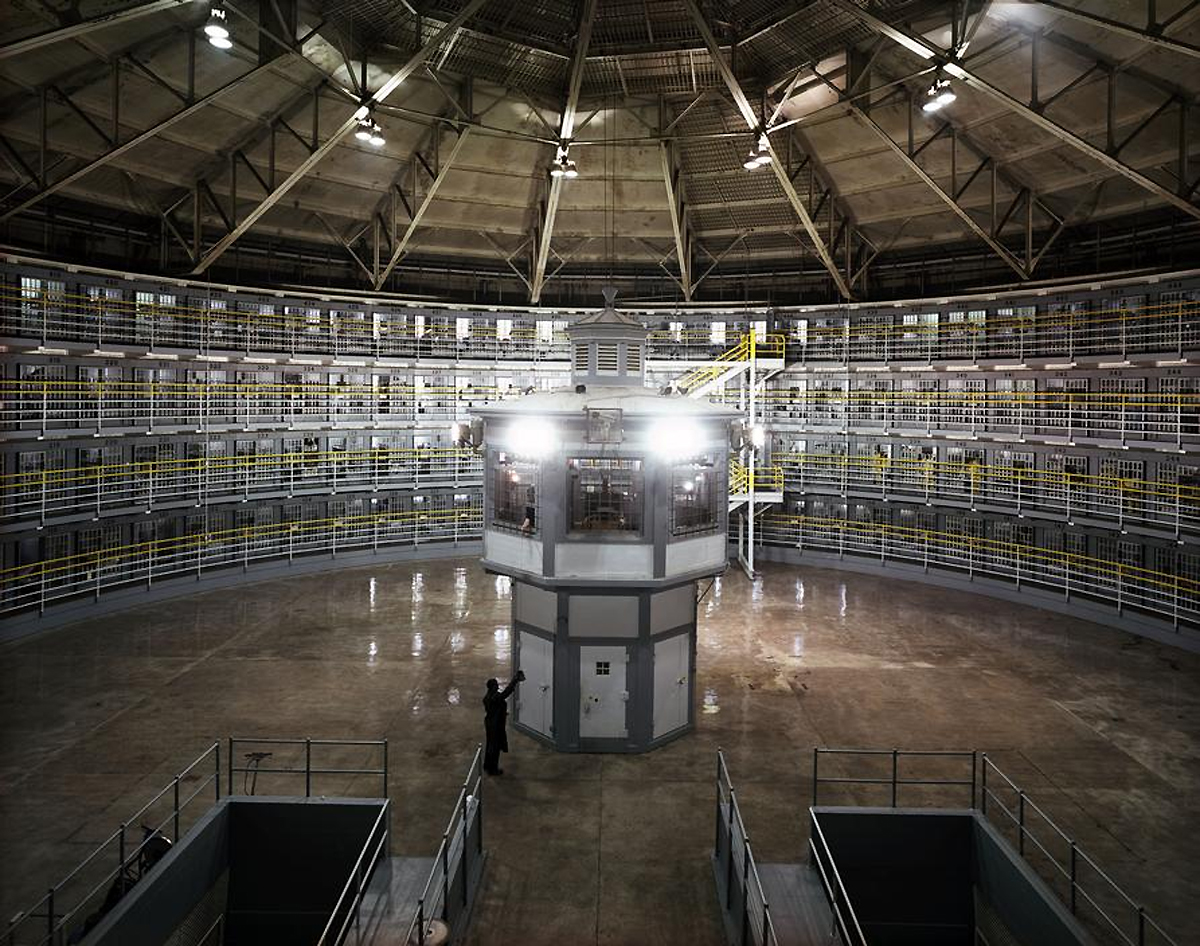
\includegraphics[width=350px]{chapters/01/images/panoptique.jpg}
    \caption{\label{panoptique}\emph{Stateville Correctional Center}, Illinois, États-Unis : Prison construite sur le modèle panoptique.}
\end{figure}

\paragraph{} On retrouvera le panoptique dans la littérature de science fiction et d'anticipation du XX\up{ème} siècle.
Dans \emph{La Zone du Dehors} \cite{Damasio0}, Alain Damasio décrit une société désindividualisante qui, à la place
de noms, attribue des matricules changants à des citoyens normés. De manière à assurer \emph{préventivement} l'ordre et la
sécurité, des tours panoptiques aux parois de verre sans tain surplombent la cité et sont accessibles à tous pour épier
et reporter en toute impunité. Cela tend alors à développer chez chacun le sentiment latent et insidieux d'être observé, 
constamment sous surveillance.

\paragraph{} C'est justement sur cet effet que vont reposer, selon Michel Foucault, les nouveaux modèles disciplinaires.
\guillemotleft Le vrai effet du Panopticon, c'est d'être tel que, même lorsqu'il n'y a personne, l'individu dans sa
cellule, non seulement se croie, mais se sache observé, qu'il ait l'expérience constante d'être dans un état de visibilité
pour le regard.\guillemotright \cite{Foucault0} Dès lors, à quoi bon recourir à la violence ? Chacun se sachant, à tort
ou à raison, observé continuellement agira en conséquence. Mais Foucault pousse plus loin son raisonnement, comparant la
panoptique pénitentiaire à un système de documentation des individus. Le geôlier peut alors prélever sans interruption
des informations et observations à propos des détenus, les analysant, les catégorisant, dans le but de \guillemotleft 
[Faire] de la peine rendue nécessaire par l'infraction une modification du détenu, utile pour la société.\guillemotright

\paragraph{} Si l'on repense à la volonté initiale de Bentham d'appliquer le modèle panoptique à toutes sortes d'institutions
(universités, hôpitaux, ...), on assiste alors à l'objectification de l'individu, qui n'est plus considéré que comme le 
n\oe{}ud du complexe maillage qu'est la \emph{Société}, entité transcendentale se nourrissant de ses - ou plutôt de 
\emph{ces} ? - individus pour évoluer, pour le meilleur comme pour le pire.

\paragraph{} Mais de quoi les sociétés sont-elles consitutées sinon d'Hommes ? De là, ce sont bien les aspirations et 
motivations de ceux qui les composent qu'elles reflètent à l'identique, et c'est justement cette volonté de contrôle que
la technologie viendra par la suite outiller. Nous sommes bien loin de l'Oasis de Pierre Rabhi, pleine de paix et de
simplicité \cite{Rabhi1}. Nous allons donc d'abord nous intéresser à l'origine du Réseau, épine dorsale de notre Moi 
numérique, sans laquelle aucun des services que nous utilisons au quotidien n'aurait pu voir le jour.


\paragraph{Historique}

\paragraph{} Les premières recherches ayant pour objectif la mise en place d'un réseau capable de résister à une frappe
nucléaire massive datent de 1957 \cite{Internet0}, quand le \emph{United States Department of Defense} (DoD) prend la
décision de fonder l'\emph{Advanced Research Projects Agency} (ARPA), un groupe scientifique ayant pour mission de concevoir
des innovations technologiques pour l'armée. Épaulés par les chercheurs de la \emph{RAND Corporation} à partir de 1962,
leurs travaux aboutiront un an plus tard sur l'ébauche d'un réseau décentralisé pouvant continuer à fonctionner dans le
cas où une ou plusieurs machines le composant viendraient à s'arrêter. L'idée d'un système décentralisé vient de Paul Baran,
qui inventa avec Donald Davies la communication de données par paquets, ajoutant ainsi à la résilience du système : le réseau
formant un maillage anarchique, chaque paquet pourra emprunter la route la plus courte possible afin de parvenir à sa 
destination, et aura la capacité de patienter durant un laps de temps maximal prédéfini s'il se trouvait dans l'incapacité
de la joindre.

\paragraph{} Le projet fut cependant refusé par l'armée, et il faudra attendre 1969, 6 ans plus tard, pour que celui-ci
se concrétise sous le nom d'\emph{Arpanet}. \emph{Bolt Beranek and Newman Inc.} (BBN) mettra en place, sur commande de
l'ARPA, un réseau reliant quatre des grands centres universitaires américains en utilisant le \emph{Network Control Protocol}
(NCP), sur des lignes pouvant atteindre 50 kilobits par seconde. Les universités concernées sont l'Université de Californie
à Los Angeles (UCLA), l'Institut de Recherche de Stanford (SRI), l'Université de Californie à Santa Barbara (UCSB) et
l'Université de l'Utah.

\begin{figure}[ht]
    \centering
    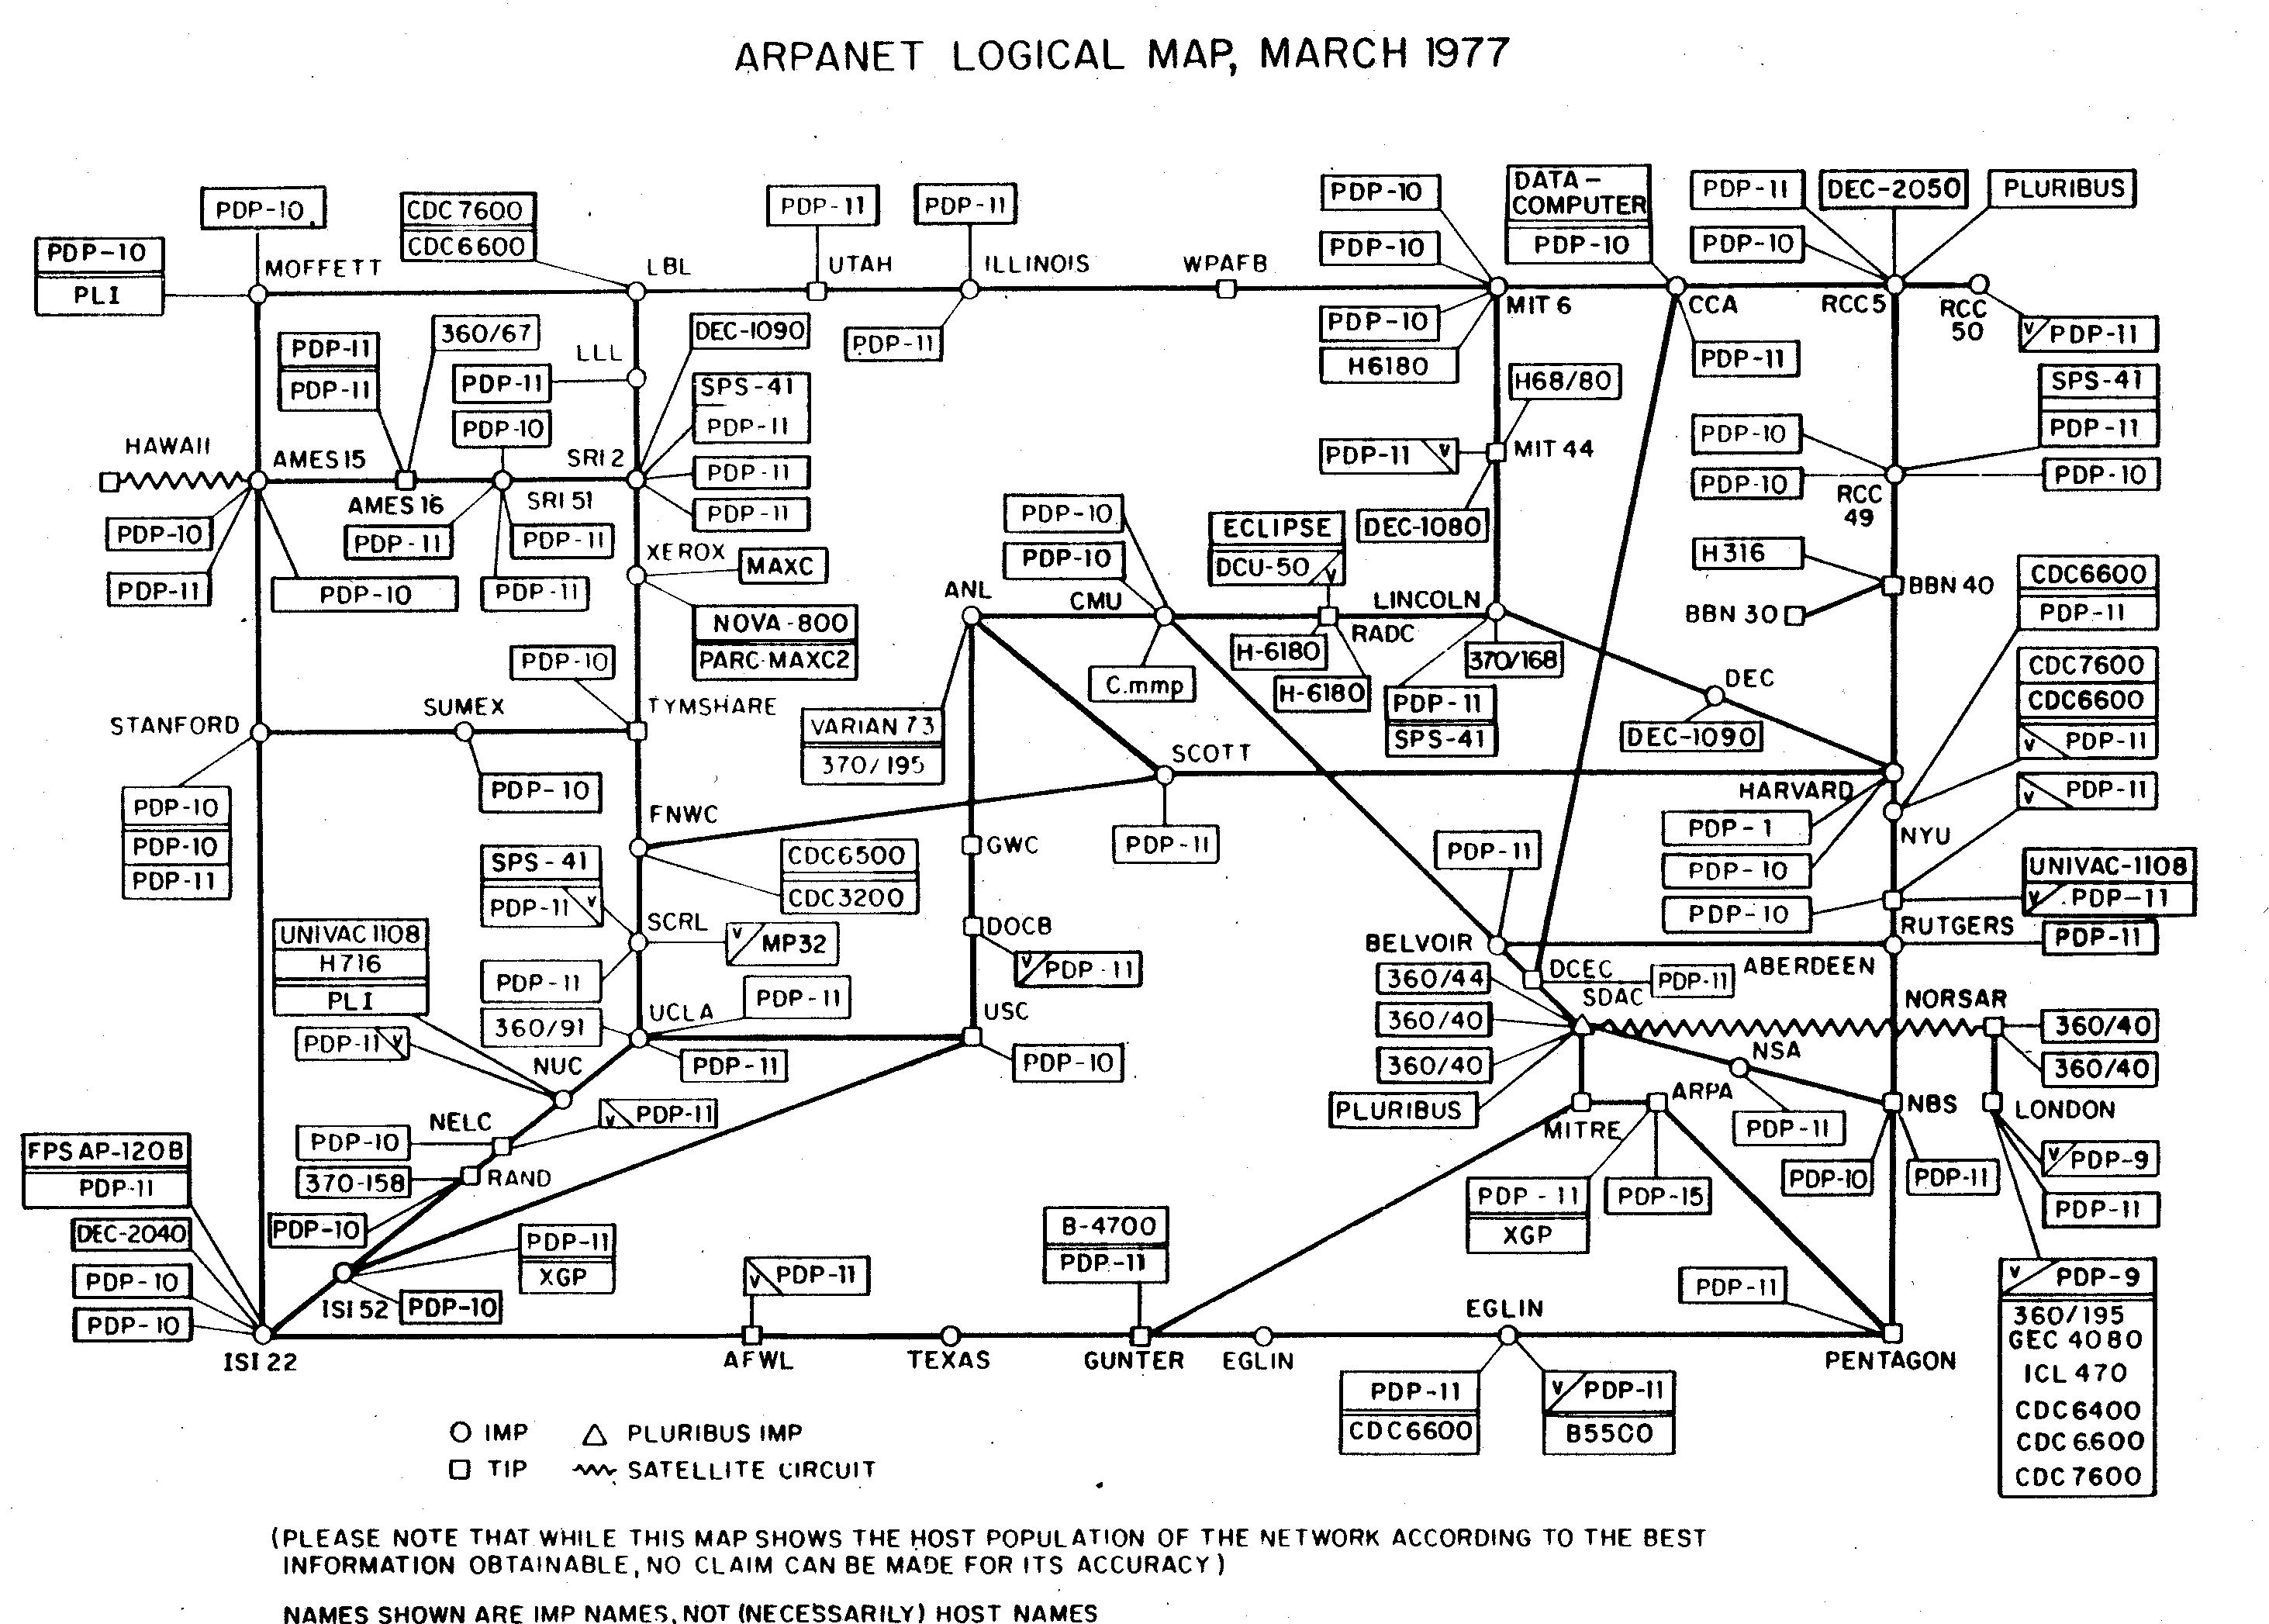
\includegraphics[width=350px]{chapters/01/images/arpanet_map.jpg}
    \caption{\label{arpanet}Carte du réseau Arpanet, mars 1977.}
\end{figure}

\paragraph{} Il faudra attendre encore deux avancées majeures pour que ce réseau soit utilisable par le grand public :
le protocole TCP/IP, et le DNS.

\paragraph{TCP/IP} La suite TCP/IP, nommée après les deux premiers protocoles qui la compose (le \emph{Transmission Control
Protocol} et l'\emph{Internet Protocol}), est développée en 1973 par Vinton Cerf et Bob Kahn. Son modèle est constitué de
quatre couches prenant en charge la transmission de données : les couches hautes manipulent les données abstraites
présentées à l'utilisateur, tandis que les couches basses permettent la représentation de ces données sur un médium
physique (aujourd'hui : connecteurs 8P8C - abusivement appelés RJ45 -, fibres optiques, ...). Adopté pour l'Arpanet en
1976 sur décision du DoD, il faudra attendre 1983 pour sa mise en place effective.

\paragraph{} Il est important aujourd'hui de bien faire la distinction entre le modèles TCP/IP et le modèle OSI 
(\emph{Open Systems Interconnection}, publié en 1984). Ce dernier, plus rigoureux, est composé de 7 couches et ne
propose pas d'interopérabilité à proprement parler avec le modèle TCP/IP. Il est utilisé presque exclusivement par des
équipements réseau.

\begin{figure}[ht]
    \centering
    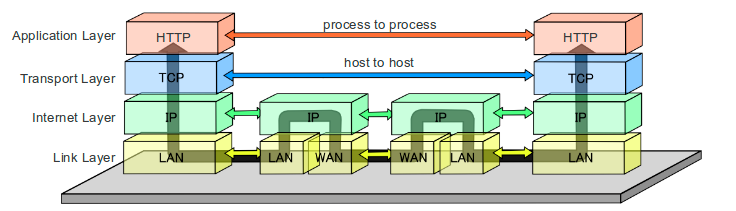
\includegraphics[width=350px]{chapters/01/images/tcpip_dataflow.png}
    \caption{\label{tcpip_dataflow}Flux de données du protocole TCP/IP.}
\end{figure}

\paragraph{DNS} Le \emph{Domain Name System} (DNS) est la solution qui a été trouvée pour résoudre les problèmes survenus
suite à l'augmentation de la popularité du réseau Arpanet. En effet, de manière à ce que les différentes machines du 
réseau puissent communiquer entre elles, il était nécessaire qu'elles maintiennent à jour un fichier \emph{hosts.txt}
permettant d'effectuer la conversion entre un nom d'hôte et l'adresse correspondante sur le réseau. En réalité, ce fichier
était maintenu à jour par le \emph{Network Information Center} (NIC) de l'institut de recherche de Stanford, qui centralisait
les modifications qui lui étaient transmises par les différents administrateurs du système et qui s'occupait de redistribuer
périodiquement le fichier mis à jour. Cependant, avec l'augmentation progressive du traffic, le NIC se retrouva dans
l'incapacité de supporter la charge réseau et des problèmes de collision de nom survinrent de plus en plus fréquemment.

\paragraph{} Jon Postel, Paul Mockapetris et Craig Partridge rédigèrent en 1983 les spécifications de ce qui devait 
devenir l'un des piliers d'Internet tel que nous le connaissons aujourd'hui : le DNS. Il s'agit d'une base de données
distribuée stockant les noms de domaines, et divisée en zones. Chacune de ces zones était prise en charge par un ou plusieurs
serveurs de noms (\emph{Name Servers}) répondant aux requêtes des résolveurs (\emph{resolvers}), petits programmes se
chargeant de transformer un nom de domaine en adresse. En 1984, les suffixes DNS, ou \emph{Top Level Domains} (TLD),
font leur apparition. Disposant chacun de leur propre zone DNS, ils permettront dans un premier temps de regrouper les
noms de domaine par fonction : \emph{.com} pour les sites commerciaux, \emph{.gov} pour les sites gouvernementaux des
États-Unis, etc. Avec le temps, certaines de ces particularités furent dépréciés (les sites en \emph{.com}
ne fournissent plus obligatoirement des services d'ordre commerciaux), et l'on vit apparaître les TLD nationaux (\emph{.fr},
\emph{.us}, \emph{.uk}, ...) dont l'obtention est soumise aux lois du pays concerné.

\paragraph{} Une fois ces systèmes mis en place, le réseau qui n'était à l'origine destiné qu'à des fins de recherche
militaire avait atteint un seuil majeur d'évolutivité. L'invention du "Web" est historiquement située en 1989 et
attribuée à Sir Timothy John Berners-Lee, alors chercheur au \emph{Conseil Européen pour la Recherche Nucléaire} (CERN)
de Genève, et à son texte \guillemotleft Information Management: A Proposal\guillemotright \cite{Internet1}. Sa volonté
est alors de mettre en place un système d'information global pour la recherche, à l'image d'Arpanet - mais accessible par tous.
Il est l'auteur d'\emph{httpd}, le premier serveur HTTP, et de \emph{WWW} (\emph{World Wide Web}), le premier client.
Il préside depuis 1994 le \emph{World Wide Web Consortium} (W3C), organisme qu'il a lui-même fondé et chargé de mettre
au point les nouveaux standards des technologies Web.

\paragraph{} Toutes les briques étaient en place pour l'adoption par le grand public : les technologies, réseaux comme
logicielles, étaient fin prêtes. Pour un rapide rappel de la chronologie évoquée ici, rendez-vous dans à l'annexe
\ref{chronology} en page \pageref{chronology}.

\paragraph{} Nous assistons depuis à une démocratisation à marche forcée des technologies dans notre quotidien. 
Interconnectés, nous le sommes de plus en plus : à tel point que les industries commes les pouvoirs politiques ne
peuvent plus ignorer ni l'usage ni les réactions des réseaux. Un battement d'ailes de papillon peut provoquer de nos
jours bien plus qu'une simple tornade.